\chapter{Alignment Procedure}
\label{ch:howtoalign}

As decribed in Section~\ref{sec:detector_config}, an analysis with \corry requires a configuration file defining which detectors are present in the setup.
This file also contains the position and rotation of each detector plane.
The Z-positions of all planes can \textbf{and must} be measured by hand in the existing test beam setup and entered in this configuration file for the analysis.
The X- and Y-positions as well as the rotations cannot be measured precisely by hand.
However, these have a strong influence on the tracking since a misalignment of a fraction of a millimeter might already correspond to a shift by multiple pixel pitches.

Consequently, an alignment procedure is needed in which the detector planes are shifted and rotated iteratively relative to the detector with \parameter{role = reference} to increase the tracking quality.
More technically, the track residuals on all planes,~i.e. the distribution of the spatial distance between the interpolated track intercept and the associated cluster on the plane need to be centered around zero and 'as narrow as possible' -- the width of the distribution depends on the tracking resolution of the telescope and is influenced by many factors such as the beam energy, the material budget of the detector planes, the distance between the detector planes, etc.
It is important to correctly set the \parameter{spatial_resolution} specified in the detector configuration file described in Section~\ref{sec:detector_config} because is defining the uncertainty on the cluster positions and therefore influences the track $\chi^2$.

This chapter provides a description of how to use the alignment features of \corry.
It also includes step-by-step instructions on how to align the detector planes for new set of test beam data.
Example configuration files can be found in the \dir{testing/} directory of the repository.
These are based on a Timepix3~\cite{timepix3} telescope with an ATLASpix~\cite{atlaspix} DUT at the CERN SPS with a pion beam of \SI{120}{GeV}.

For the alignment of the \textbf{reference telescope} and \textbf{device-under-test (DUT)}, the following modules are available in \corry.
\begin{itemize}
\item \module{Prealignment} for both telescope and DUT prealignment (see Section~\ref{prealignment}).
\item \module{AlignmentTrackChi2} used for telescope alignment (see Section~\ref{alignmenttrackchi2}) and is relatively robust against an initial misalignment but usually needs several iterations.
\item \module{AlignmentMillepede}, an alternative telescope alignment algorithm (see Section~\ref{alignmentmillepede}) which requires fewer iterations to reach a precise alignment but needs a better prealignment.
\item \module{AlignmentDUTResidual} used for DUT alignment (see Section~\ref{alignmentdutresidual}).
\end{itemize}

The general procedure that needs to be followed for a successful alignment is outlined here and explained in detail below.
\begin{enumerate}
\item Prealignment of the telescope (ignoring the DUT).
\item Alignment of the telescope (ignoring the DUT).
\item Prealignment of the DUT (telescope geometry is frozen).
\item Alignment of the DUT (telescope alignment is frozen).
\end{enumerate}

\begin{warning}
When using the alignment modules, the new geometry is written out to a new geometry file which needs to be specified using the parameter \parameter{detectors_file_updated}.
For details, see Section~\ref{sec:framework_parameters}.
\end{warning}

\paragraph{Correlation vs. Residual}

A spatial \textbf{correlation} plot is filled with the spatial difference of any cluster on a given detector plane minus the position of any cluster on the reference plane. No tracking is required to fill these histograms.

A spatial \textbf{residual} plot shows the difference of the interpolated track intercept onto a given plane minus the position of its associated cluster.\\

Consequently, the goal of the alignment is to force the \textbf{residuals} to be centered around zero.
The \textbf{correlations} do not necessarily have to be centered at zero as a possible offset reflects the \emph{physical displacement} of a detector plane in X and Y with respect to the reference plane.
However, it can be useful to inspect the \textbf{correlation} plots especially in the beginning when the alignment is not yet good enough for a reasonable tracking.

\section{Aligning the Telescope}
\label{sec:align_tel}
Initially, the telescope needs to be aligned.
For this, the DUT is ignored.

\subsection*{Prealignment of the Telescope}
The \module{AlignmentTrackChi2} module requires a careful prealignment. Otherwise it does not converge and the alignment will fail.
The Z-positions of all planes need to be measured by hand \textbf{in the existing test beam setup} and then adjusted in the detectors file.
For X and Y, the alignment file from an already aligned run with the same telescope plane arrangement is a solid basis to start from.
If no previous alignment is available, all values for X and Y should be set to 0.

For the prealignment, two strategies can be applied:
\begin{itemize}
\item The \module{Prealignment} module can be used (see Section~\ref{prealignment}).
\item If the above does not bring the expected result, a manual prealignment can be performed as described below.
\end{itemize}

To have a first look at the initial alignment guess, one can run
\begin{verbatim}
$ /path/to/corryvreckan/bin/corry                     \
    -c analyse_telescope.conf                         \
   [-o detectors_file=<detectorsFile>                 \
    -o histogram_file=<histogramFile>                 \
    -o EventLoaderTimepix3.input_directory=<inputDir>]
\end{verbatim}

The \parameter{spatial_cut_abs/rel} in \module{Tracking4D} should be set to multiple ($\sim4$) pixel pitch.

One can inspect the spatial correlations in X and Ythe track $\chi^2$, and the residuals with the online monitoring or by opening the generated ROOT file after finishing the script.
These can be found in the modules \module{Correlations} (see Section~\ref{correlations}) and \module{Tracking4D} (see Section~\ref{tracking4d}).

To save time, one can limit the number of processed tracks. For instance, set \parameter{number_of_events = 10000} or \parameter{number_of_tracks = 10000} (see Section~\ref{sec:framework_parameters}).

If no peak at all is apparent in the correlations or residuals, the hitmaps can be checked to see if valid data is actually available for all planes.

Now, the \texttt{[Prealignment]} module can be used.
To prealign only the telescope, the DUT can be excluded by using \parameter{type = <detector_type_of_telescope>} (e.g.~\parameter{CLICPIX2}). For details, see Section~\ref{sec:module_manager}.

To use the module, \file{align_tel.conf} needs to be edited such that \texttt{[Prealignment]} is enabled and \texttt{[Alignment]} is disabled:
\begin{minted}[frame=single,framesep=3pt,breaklines=true,tabsize=2,linenos]{ini}
...
[Prealignment]
type = <detector_type_of_telescope> # <-- optional!
[Ignore]
#[AlignmentTrackChi2]
log_level=INFO
iterations = 4
align_orientation=true
align_position=true
\end{minted}

Then one can run
\begin{verbatim}
$ /path/to/corryvreckan/bin/corry                      \
    -c align_telescope.conf                            \
   [-o detectors_file=<detectorsFile>                  \
    -o detectors_file_updated=<detectorsFileUpdated>   \
    -o histogram_file=<histogramFile>                  \
    -o EventLoaderTimepix3.input_directory=<inputDir>]
\end{verbatim}

The actual prealignment is only performed after the events have been analyzed and written to the detectors file in the finalizing step.
This means to check whether the alignment has improved, one needs to re-run the analysis or the next iteration of the alignment as the previously generated ROOT file corresponds to the initial alignment.
This is the case for every iteration of the prealignment or alignment.

Generally, it suffices to run the \texttt{[Prealignment]} module once and then proceed with the next step.

\subsubsection*{Manual Prealignment of the Telescope}
If the prealignment using the module \texttt{[Prealignment]} does not bring the expected results, one can also perform the same steps manually by investigating the residuals of the DUT with respect to tracks.
For the residuals, the shift of the peak from 0 can be estimated with a precision of $\mathcal{O}(\SI{100}{\micro m})$ by zooming in using the \texttt{TBrowser}.
For instance, if the peak is shifted by +\SI{+300}{\micro m}, the detectors file needs to be edited and \SI{+300}{\micro m} should be added to the respective position, if \SI{-300}{\micro m}, subtracted.

After modifying the positions of individual planes in the configuration file, \corry can be re-run to check the correlation and residual plots for the updated geometry.
These steps need to be iterated a few times until the peaks of the \textbf{residuals} are centered around 0.

Rotational misalignments can be inferred from the slope of the 2D spatial correlation plots, the actual rotation angle has to be calculated using the respective pixel pitches of the devices.

\begin{warning}
It is important \textbf{not} to force the peak of the spatial \textbf{correlations} to be at exactly 0 because the position of the peak corresponds to the \textit{physical displacement} of a detector plane in X and Y with respect to the reference plane.
The spatial \textbf{correlations} should \textbf{only be used} if the spatial \textbf{residual} plots are not filled reasonable due to bad tracking.
Hence, the spatial correlations can be shifted towards zero in a first iteration.
\end{warning}


\subsection*{Alignment of the Telescope}
After the prealignment, the actual \textbf{precise} alignment can be performed using the \texttt{[AlignmentTrackChi2]} module (see Section~\ref{alignmenttrackchi2}).
To this end, \file{align_tel.conf} needs to be modified such that the prealignment is disabled and the alignment is enabled:
\begin{minted}[frame=single,framesep=3pt,breaklines=true,tabsize=2,linenos]{ini}
...
#[Prealignment]
#[Ignore]
[AlignmentTrackChi2]
log_level=INFO
iterations = 4
align_orientation=true
align_position=true
\end{minted}

The algorithm performs an optimisation of the track $\chi^2$.

Typically, the alignment needs to be iterated a handful of times until the residuals (which again can be inspected in the ROOT file after re-running the analysis) are nicely centered around 0 and 'as narrow as possible' -- the RMS of the residuals corresponds to the spatial resolution of each plane (convolved with the resolution of the telescope) and should thus be $\lesssim$ pixel pitch$/\sqrt{12}$.
Starting with a \parameter{spatial_cut_abs/rel} in \texttt{[Tracking4D]} (see Section~\ref{tracking4d}) of multiple ($\sim4$) pixel pitches, it should be decreased incrementally down to the pixel pitch (e.g. run \SI{200}{\micro\m} twice, then run \SI{150}{\micro\m} twice, then \SI{100}{\micro\m} twice, and then \SI{50}{\micro\m} twice).
This allows to perform the alignment with a tight selection of very high quality tracks only.
Also the \parameter{max_track_chi2ndof} should be decreased for the same reason.
For the further analysis, the cuts can be released again.

It may happen that the procedure runs into a 'false minimum', i.e. it converges in a wrong alignment in which the residuals are clearly not centered around 0.
In this case, it is required to go one step back and improve the prealignment.

Once the alignment is done, one should obtain narrow residuals centered around 0 and a good distribution of the track $\chi^2$ as shown in Figures~\ref{fig:exampleAlignment}.
If the alignment keeps to fail, it is possible to allow only for rotational or translational alignment while freezing the other for one or a few iterations.

\begin{minted}[frame=single,framesep=3pt,breaklines=true,tabsize=2,linenos]{ini}
...
#[Prealignment]
#[Ignore]
[AlignmentTrackChi2]
log_level=INFO
iterations = 4
align_orientation=false #<-- disable rotational alignment
align_position=true
\end{minted}

\begin{figure}
    \centering
    \begin{subfigure}[t]{0.66\textwidth}
        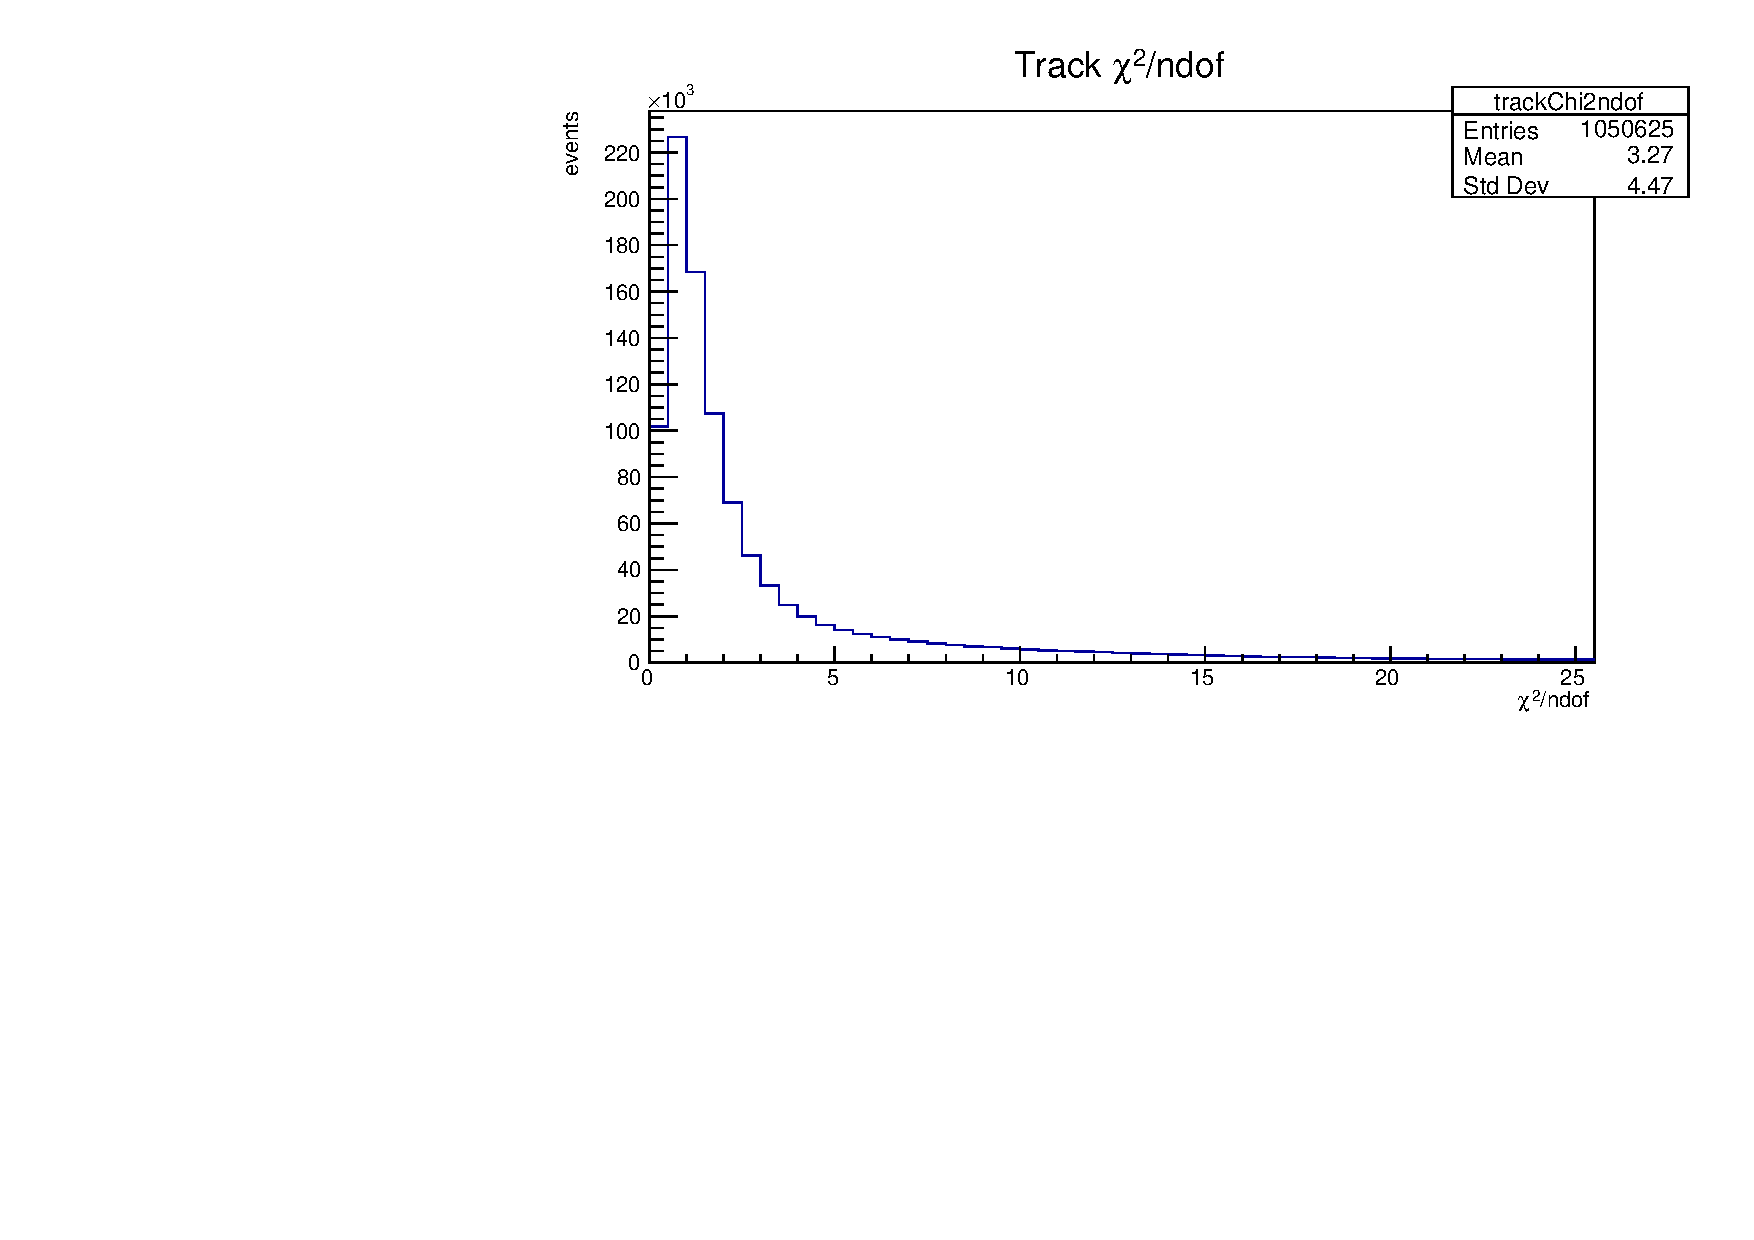
\includegraphics[width=\textwidth]{trackChi2ndof_goodexample}
        \caption{Good example of a track $\chi^2$/ndf distribution.}
        \label{fig:trackChi2}
    \end{subfigure}
    \begin{subfigure}[t]{0.66\textwidth}
        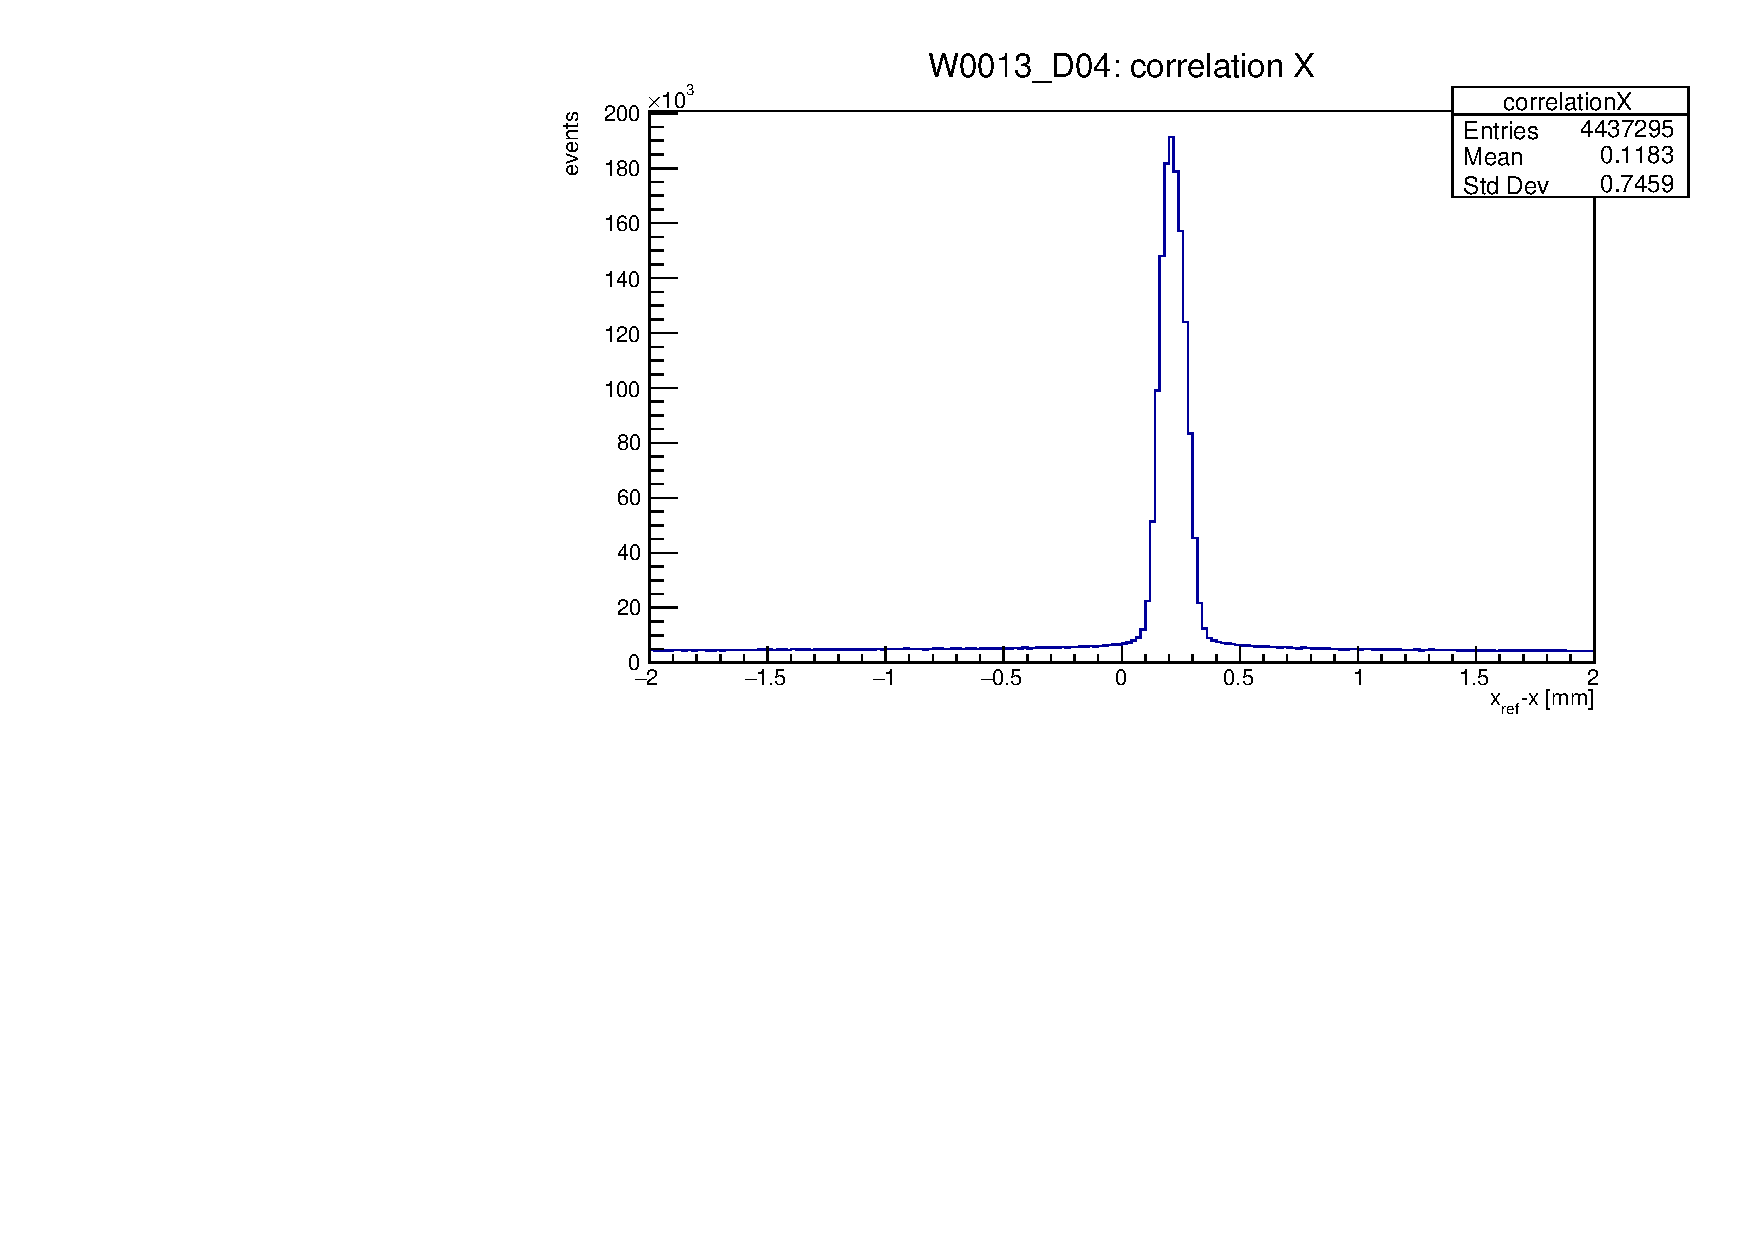
\includegraphics[width=\textwidth]{correlationX_goodexample}
        \caption{Good example of a spatial correlation plot between two telescope planes. The offset from zero corresponds to the \emph{physical displacement} of the plane  with respect to the reference plane.}
        \label{fig:correlationX}
    \end{subfigure}
    \begin{subfigure}[t]{0.66\textwidth}
        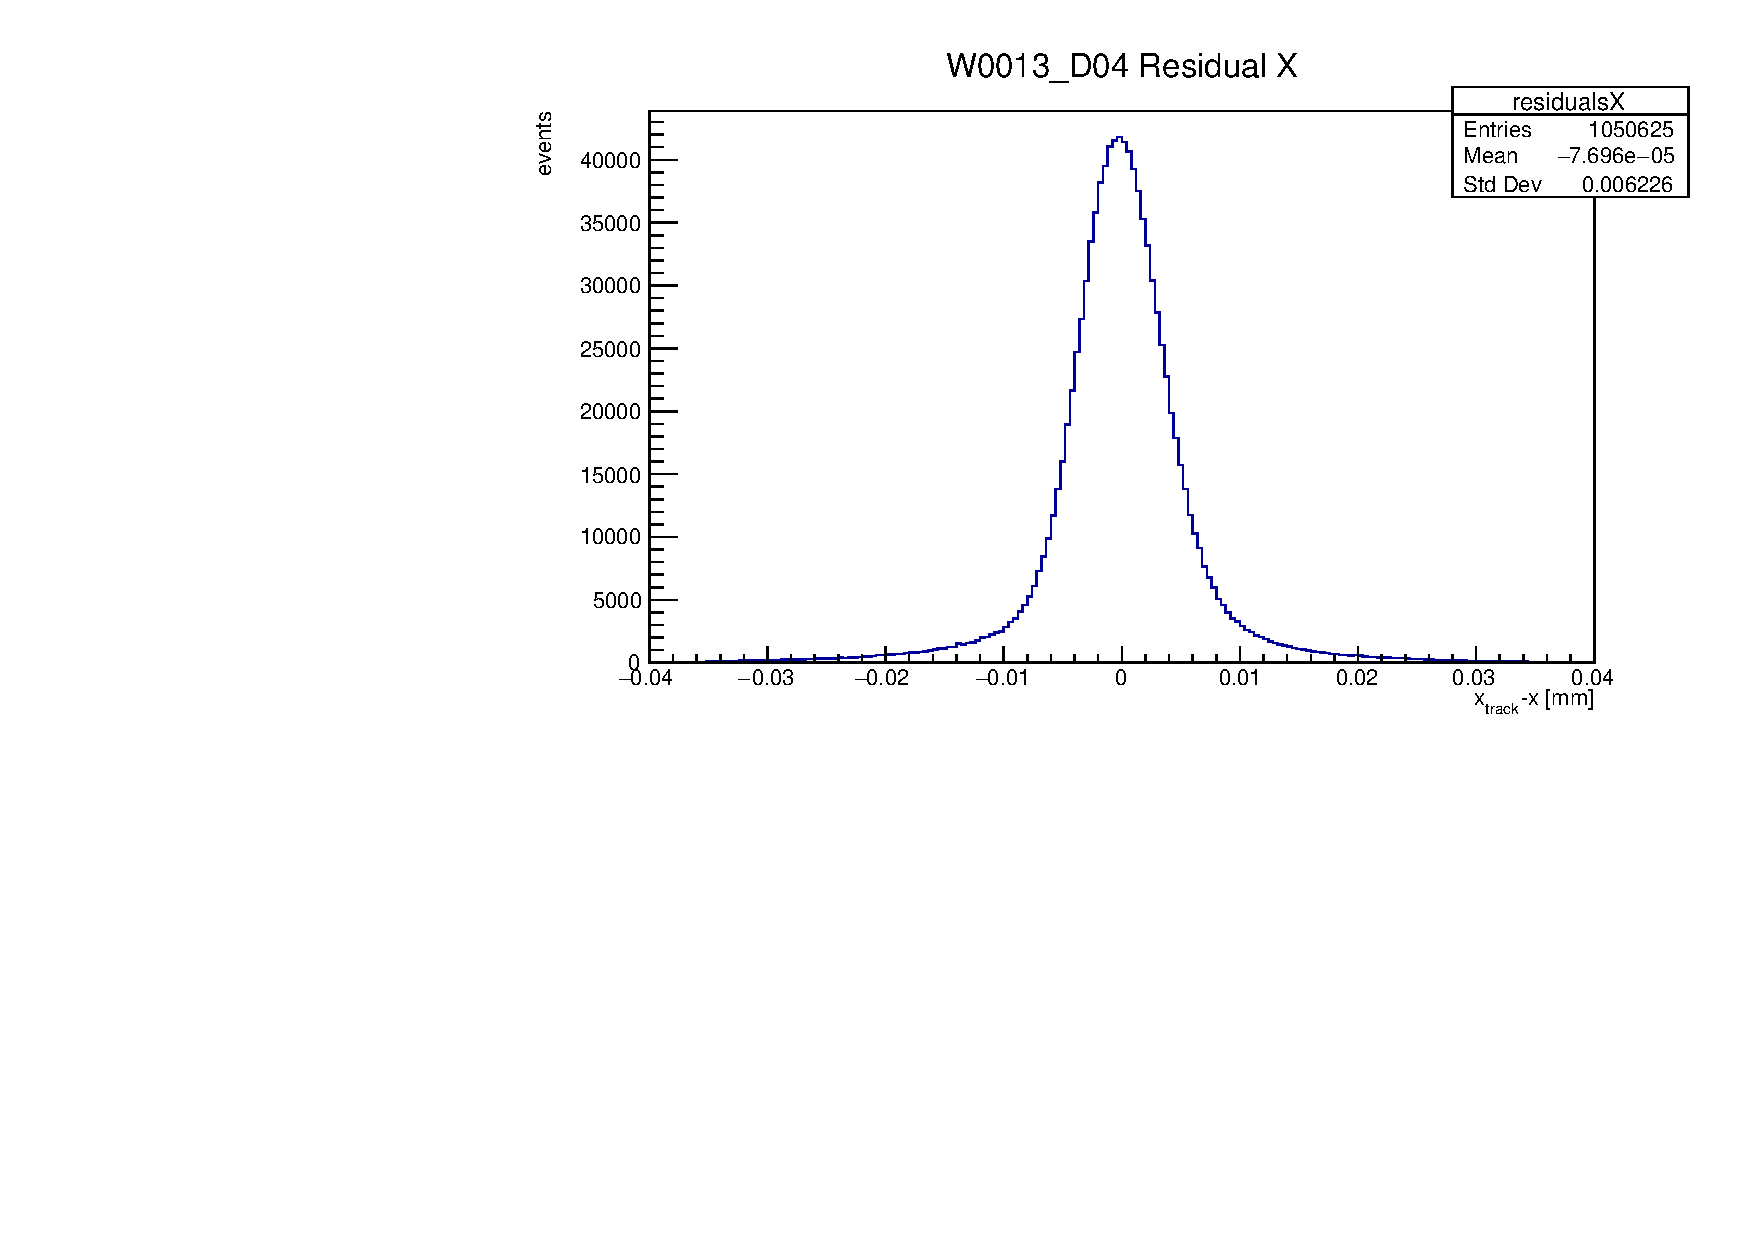
\includegraphics[width=\textwidth]{residualX_goodexample}
        \caption{Good example of a spatial residual distribution. It is centered around zero.}
        \label{fig:residualX}
    \end{subfigure}
    \caption{Examples of distributions how they should look after a successful alignment of the Timepix3 telescope at the CERN SPS with \SI{120}{\GeV} pions.}
    \label{fig:exampleAlignment}
\end{figure}

Instead of using \texttt{[AlignmentTrackChi2]}, one can also use the module \texttt{[AlignmentMillepede]} (see Section~\ref{alignmentmillepede}).
It allows a simultaneous fit of both the tracks and the alignment constants.
The modules stops if the convergence, i.e.~the absolute sum of all corrections over the total number of parameters, is smaller than the configured value, and the aligment is complete.
It should be noted that this module requires a rather good prealignment already.

\section{Aligning the DUT}
\label{sec:align_dut}
Once the telescope is aligned, its geometry is not changed anymore. From now on, it is used to build tracks which are then matched to clusters on the DUT.

\subsection*{Prealignment of the DUT}
The prealignment of the DUT follows the same strategy as for the telescope. To look at the current alignment, the script
\begin{verbatim}
$ /path/to/corryvreckan/bin/corry                          \
    -c analyse_atlaspix.conf                               \
   [-o detectors_file=<detectorsFile>                      \
    -o histogram_file=<histogramFile>                      \
    -o EventLoaderTimepix3.input_directory=<inputDir_TPX>  \
    -o EventLoaderATLASpix.input_directory=<inputDir_APX>]
\end{verbatim}
needs to be run.
If no better guess is available, the initial alignment of the DUT should be set to $x=y=0$.

Then, by repeatedly running \corry and modifying the position of the DUT in the detectors file one should be able to bring the peaks of the spatial residuals in X and Y close to zero.
If no peak at all can be seen in the residual plots, the spatial correlations plots can be inspected. In addition, potentially parameters related to the corresponding event loader need to be corrected in the configuration file.

\begin{warning}
If using the \texttt{[Prealignment]} module, it is possible to prealign all planes at once as described above in Section~\ref{sec:align_tel}.
If only the DUT shall be prealigned here, the parameter \parameter{name = <name_of_dut>} or \parameter{type = <detector_type_of_dut>} need to be used.
Otherwise, the telescope planes are also shifted again destroying the telescope alignment.
\end{warning}

\begin{minted}[frame=single,framesep=3pt,breaklines=true,tabsize=2,linenos]{ini}
...
[Prealignment]
name = <name_of_dut> # <-- otherwise the telescope planes will be moved!

[Ignore]
#[AlignmentDUTResiduals]
log_level=INFO
iterations = 4
align_orientation=true
align_position=true
\end{minted}

\subsection*{Alignment of the DUT}
The alignment strategy for the DUT is similar as for the telescope and requires multiple iterations.
In \file{align_dut.conf}, the prealignment needs to be disabled and the alignment enabled.
Now, the algorithm optimizes the residuals of the tracks through the DUT.

\begin{minted}[frame=single,framesep=3pt,breaklines=true,tabsize=2,linenos]{ini}
...
#[Prealignment]
#[Ignore]
[AlignmentDUTResiduals]
log_level=INFO
iterations = 4
align_orientation=true
align_position=true
\end{minted}

Then run
\begin{verbatim}
$ /path/to/corryvreckan/bin/corry                          \
    -c align_dut.conf                                      \
   [-o detectors_file=<detectorsFile>                      \
    -o detectors_file_updated=<detectorsFileUpdated>       \
    -o histogram_file=<histogramFile>                      \
    -o EventLoaderTimepix3.input_directory=<inputDir_TPX>  \
    -o EventLoaderATLASpix.input_directory=<inputDir_APX>]
\end{verbatim}

Like for the telescope alignment, the RMS of the residuals can be interpreted as the spatial resolution of the DUT (convolved with the track resolution of the telescope at the position if the DUT) and should thus be $\lesssim$~pixel pitch$/\sqrt{12}$.
Again, starting with a \parameter{spatial_cut_abs/rel} in \texttt{[DUTAssociation]} (see Section~\ref{dutassociation}) of multiple ($\sim4$) pixel pitches, it should be decreased incrementally down to the pixel pitch. Note that an asymmetric pixel geometry requires the \parameter{spatial_cut_abs/rel} to be chosen accordingly.

If the alignment keeps to fail, it is possible to allow only for rotational or translational alignment while freezing the other for one or a few iterations.

\begin{minted}[frame=single,framesep=3pt,breaklines=true,tabsize=2,linenos]{ini}
...
#[Prealignment]
#[Ignore]
[AlignmentDUTResiduals]
log_level=INFO
iterations = 4
align_orientation=false #<-- disable rotational alignment
align_position=true
\end{minted}
